% !TeX root = ./report.tex
% !TeX encoding = UTF-8 Unicode
% !TeX spellcheck = it_IT
% !TeX program = arara
% !TeX options = --log --verbose --language=it "%DOC%"

% arara: lualatex:      { interaction: batchmode }
% arara: lualatex:      { interaction: nonstopmode, synctex: yes }

\documentclass[a4paper,11pt,notitlepage,final]{scrartcl}

\usepackage{fancyvrb}

\begin{VerbatimOut}{\jobname.xmpdata}
\Title{Fertility Dataset Analysis}
\Author{Niccolò Maltoni}
\Copyright{Questo documento è fornito sotto licenza Creative Commons Attribution-ShareAlike 4.0 International}
\CopyrightURL{http://creativecommons.org/licenses/by-sa/4.0}
\end{VerbatimOut}

\usepackage[english,italian]{varioref}

\usepackage[luatex,dvipsnames,table,xcdraw]{xcolor}
\usepackage[a-1b]{pdfx}

%% Font
\usepackage{fontspec}
\defaultfontfeatures{Ligatures=TeX}
\setmainfont[SmallCapsFont={* Caps}]{Latin Modern Roman}
\setsansfont{Latin Modern Sans}

%% Matematica
\usepackage{amsmath}
\usepackage[math-style=ISO]{unicode-math}
\setmathfont{Latin Modern Math}
\usepackage[output-decimal-marker={,},binary-units]{siunitx}

\defaultfontfeatures{} % reset per mono font
\setmonofont{Latin Modern Mono}

%% Lingue
\usepackage[strict=true,autostyle=true,english=american,italian=guillemets]{csquotes}
\usepackage{polyglossia}
\setmainlanguage[babelshorthands]{italian}
\setotherlanguage[variant=american]{english}

%% Altri pacchetti
\usepackage{graphicx}
\graphicspath{{fig}}
\usepackage{xargs}
\usepackage[colorinlistoftodos,prependcaption,textsize=tiny]{todonotes}
\newcommandx{\unsure}[2][1=]{\todo[linecolor=red,backgroundcolor=red!25,bordercolor=red,#1]{#2}}
\newcommandx{\change}[2][1=]{\todo[linecolor=blue,backgroundcolor=blue!25,bordercolor=blue,#1]{#2}}
\newcommandx{\info}[2][1=]{\todo[linecolor=OliveGreen,backgroundcolor=OliveGreen!25,bordercolor=OliveGreen,#1]{#2}}
\newcommandx{\improvement}[2][1=]{\todo[linecolor=Plum,backgroundcolor=Plum!25,bordercolor=Plum,#1]{#2}}
\newcommandx{\thiswillnotshow}[2][1=]{\todo[disable,#1]{#2}}
\usepackage{subcaption}
\usepackage{caption}
\usepackage{scrhack}
\usepackage{float}

\usepackage{geometry}
\geometry{a4paper,heightrounded}
\usepackage{setspace}
\onehalfspacing{}

% \usepackage[maxcitenames=2,mincitenames=2,maxbibnames=99,minbibnames=99,style=ieee,giveninits=true,backend=biber]{biblatex}
% \addbibresource{biblio.bib}

% \usepackage[htt]{hyphenat}
% \usepackage{enumerate}

\usepackage{xurl}
\usepackage{microtype}

\hypersetup{%
  pdfpagemode={UseNone},
  hidelinks,
  hypertexnames=false,
  linktoc=all,
  unicode=true,
  pdftoolbar=false,
  pdfmenubar=false,
  plainpages=false,
  breaklinks,
  pdfstartview={Fit},
  pdflang={it}
}

\usepackage[english,italian,nameinlink]{cleveref}

\title{\LARGE{\textbf{Fertility Dataset Analysis}}}

\author{Niccolò~Maltoni}

\date{%
  \small{Data Mining}\\%
  \small{Anno accademico 2019--2020}
}

\begin{document}

\maketitle

\section{Introduzione}\label{sec:intro}

Per la produzione dell'elaborato, si è scelto di condurre le operazioni di studio e mining dei dati sul dataset chiamato \emph{Fertility Data Set}\footnote{\url{http://archive.ics.uci.edu/ml/datasets/Fertility}\label{note:dataset}}, prelevato dal sito \emph{UCI Machine Learning}.
In questa \nameCref{sec:intro} verranno presentati il dataset sul quale è stato svolto il lavoro.
Verrà preso in considerazione il dominio di provenienza del dataset e la struttura dei dati in esso contenuti prima di apportarne delle modifiche,
per poter essere in grado di dedurre conoscenza dai dati in questione.

\subsection{Descrizione del dominio}\label{subsec:intro:domain}

Il dataset contiene i risultati degli esami di fertilità effettuati su campioni di seme secondo i criteri dell'Organizzazione Mondiale della Sanità (\emph{World Health Organization 2010});
l'analisi sul seme maschile permettono infatti di individuare potenziali problemi di sterilità nei pazienti.

La possibilità di alterazioni del seme possono essere correlate ad aspetti diversi della vita dell'individuo:
oltre alla genetica, pare che la sterilità maschile possa essere correlata anche a fattori socio-demografici, ambientali e di stile di vita.

Può essere interessante analizzare quanto effettivamente la presenza di malattie e traumi non necessariamente locali all'apparato genitale possano incidere sulla fertilità del paziente,
come anche uno stile di vita particolarmente sedentario o il consumo abituale di sostanze non ritenute particolarmente salutari come tabacco da fumo e alcool.
In questo modo, tramite Data Mining sarebbe possibile aiutare la diagnosi medica tramite il supporto informatico.

% Fertility rates have dramatically decreased in the last two decades, especially in men.
% It has been described that environmental factors, as well as life habits, may affect semen quality.
% Artificial intelligence techniques are now an emerging methodology as decision support systems in medicine.
% In this paper we compare three artificial intelligence techniques, decision trees, Multilayer Perceptron and Support Vector Machines,
% in order to evaluate their performance in the prediction of the seminal quality from the data of the environmental factors and lifestyle.\label{xxx}
% To do that we collect data by a normalized questionnaire from young healthy volunteers and then, we use the results of a semen analysis to asses the accuracy in the prediction of the three classification methods mentioned above.
% The results show that Multilayer Perceptron and Support Vector Machines show the highest accuracy, with prediction accuracy values of 86\% for some of the seminal parameters.
% In contrast decision trees provide a visual and illustrative approach that can compensate the slightly lower accuracy obtained.
% In conclusion artificial intelligence methods are a useful tool in order to predict the seminal profile of an individual from the environmental factors and life habits.
% From the studied methods, Multilayer Perceptron and Support Vector Machines are the most accurate in the prediction.
% Therefore these tools, together with the visual help that decision trees offer, are the suggested methods to be included in the evaluation of the infertile patient.

\subsection{Descrizione del dataset}\label{subsec:intro:dataset}

Questo dataset contiene i risultati degli esami di fertilità di 100 uomini;
il risultato di questi esami può essere di due tipologie, \emph{normale} oppure \emph{alterato}, che indica un potenziale problema di sterilità nel paziente.
Questi risultati sono correlati all'interno del dataset con altri dati di natura socio-demografica, ambientale e abitudinaria dei soggetti analizzati.

Il file \href{http://archive.ics.uci.edu/ml/machine-learning-databases/00244/fertility_Diagnosis.txt}{\texttt{fertility\_Diagnosis.txt}}
contiene l'intero dataset, costituito da linee costituenti i record, con gli attributi separati da virgole.
Al suo interno, sono presenti \emph{100 istanze} composte di \emph{10 attributi};
di seguito sono riportati con una breve descrizione.

\begin{description}
  \item[Stagione]
    Attributo nominale che rappresenta la stagione in cui è stato svolto l'esame.
    Può assumere quattro possibili valori, corrispondenti alle stagioni astronomiche dell'anno solare:
    \begin{itemize}
      \item \(-1\): \emph{primavera};
      \item \(-0.33\): \emph{estate};
      \item \(0.33\): \emph{autunno};
      \item \(1\): \emph{inverno}.
    \end{itemize}
  \item[Età]
    Attributo numerico che rappresenta l'età dei partecipanti al test al momento dell'analisi.
    Può assumere valori numerici in un range compreso tra \(0.5\) (corrispondente a 18 anni) e \(1\) (corrispondente a 36 anni).
  \item[Malattie infantili]
    Attributo binario che rappresenta la presenza o meno di patologie clinicamente rilevanti (\emph{Varicella}, \emph{Orecchioni}, \emph{Morbillo}, etc.) contratte dal paziente durante l'infanzia.
    Può assumere i valori \(0\) (sì) e \(1\) (no).
  \item[Incidenti o traumi seri]
    Attributo binario che rappresenta la presenza o meno di traumi/incidenti rilevanti nella storia clinica del paziente.
    Può assumere i valori \(0\) (sì) e \(1\) (no).
  \item[Interventi chirurgici]
    Attributo binario che rappresenta la presenza o meno di interventi chirurgici nella storia clinica del paziente.
    Può assumere i valori \(0\) (sì) e \(1\) (no).
  \item[Febbre]
    Attributo nominale che rappresenta l'aver contratto, da parte del candidato, febbri particolarmente alte nell'ultimo anno.
    Può assumere tre possibili valori, corrispondenti al periodo:
    \begin{itemize}
      \item \(-1\): \emph{meno di tre mesi} dalla data dell'analisi;
      \item \(0\): \emph{più di tre mesi} dalla data dell'analisi;
      \item \(1\): \emph{mai nell'ultimo anno}.
    \end{itemize}
  \item[Consumo di alcool]
    Attributo nominale che rappresenta la frequenza del consumo di alcool, del soggetto in analisi.
    Può assumere cinque valori:
    \begin{itemize}
      \item \(0.2\): \emph{più volte al giorno};
      \item \(0.4\): \emph{una volta al giorno};
      \item \(0.6\): \emph{più volte alla settimana};
      \item \(0.8\): \emph{una volta a settimana};
      \item \(1\): \emph{molto raramente o mai}.
    \end{itemize}
  \item[Fumo]
    Attributo nominale che rappresenta le abitudini del soggetto rispetto al fumo.
    Può assumere tre valori:
    \begin{itemize}
      \item \(-1\): \emph{non fumatore};
      \item \(0\): \emph{fumatore sporadico};
      \item \(1\): \emph{fumatore abituale}.
    \end{itemize}
  \item[Ore spese seduto]
    Attributo numerico che quantifica le ore trascorse seduto al giorno dal soggetto.
    Può assumere valori numerici in un range compreso tra \(0.06\) (corrispondente a un'ora) e \(1\) (16 ore).
  \end{description}

Oltre agli attributi sopra riportati, i record del dataset sono etichettati con un attributo classe corrispondente alla diagnosi:
il carattere \texttt{N} corrisponde ad una situazione clinica \emph{normale}, mentre \texttt{O} corrisponde ad una diagnosi \emph{alterata}.

\subsection{Breve analisi dei dati}\label{subsec:intro:analysis}

Come detto nella \Vref{subsec:intro:dataset}, il dataset contiene i risultati degli esami di fertilità di 100 uomini.
Poiché il risultato di questi esami può essere di due tipologie, il problema delineato può essere affrontato come un quesito di classificazione binaria:
si deve infatti poter costruire un modello che, dati certi parametri per gli attributi presi in causa, permetta di prevedere un potenziale problema di fertilità o meno.

Gli attributi presi in considerazione sono di natura molto diversa tra loro e non tutti di banale correlazione per un non esperto del dominio, dunque molta attenzione è richiesta in questo senso.


\section{Preprocessing dei dati}

In questa sezione vengono applicate trasformazioni ai dati al fine di aumentare la qualità dell'output dei vari algoritmi e di garantire delle performance migliori.

Non si è ritenuto necessario aggregare o eliminare attributi, in quanto il numero di questi è molto ridotto e non sono presenti attributi linearmente dipendenti tra di loro.

\subsection{Importazione in Weka}

Tutte le analisi sui dati sono state effettuate tramite il software Weka\footnote{\url{https://www.cs.waikato.ac.nz/ml/weka/}}.

Il file, come detto nella \Vref{subsec:intro:dataset}, è di fatto un CSV senza linea di \emph{header}.
Purtroppo, forzando l'import del file come CSV senza effettuare modifiche non ha funzionato, anche mettendo a \texttt{true} il flag \texttt{noHeaderRowPresent};
si è dunque proceduto aggiungendo manualmente al file una linea di intestazione con i nomi delle colonne, risolvendo il problema.



\subsection{Pulizia}
\subsection{Normalizzazione}
\subsection{Campionamento}
\subsection{Discretizzazione}


\section{Analisi dei dati e classificatori utilizzati}

In questa sezione verrà riportato lo studio effettuato sul dataset.
% Ogni sottosezione tratterà di uno specifico classificatore, dei suoi risultati e degli esperimenti fatti per migliorarne il modello.

\subsection{Considerazioni sugli attributi}

Studiando la composizione dei dati per selezionare le principali tecniche da applicare,
la prima cosa che risulta visibile all'apertura del dataset è sicuramente il suo sbilanciamento nelle classi di output:
come mostrato in~\Cref{fig:classes}, su 100 pazienti in esame, solo 12 risultano compromessi.

\begin{figure}[H]
  \centering
  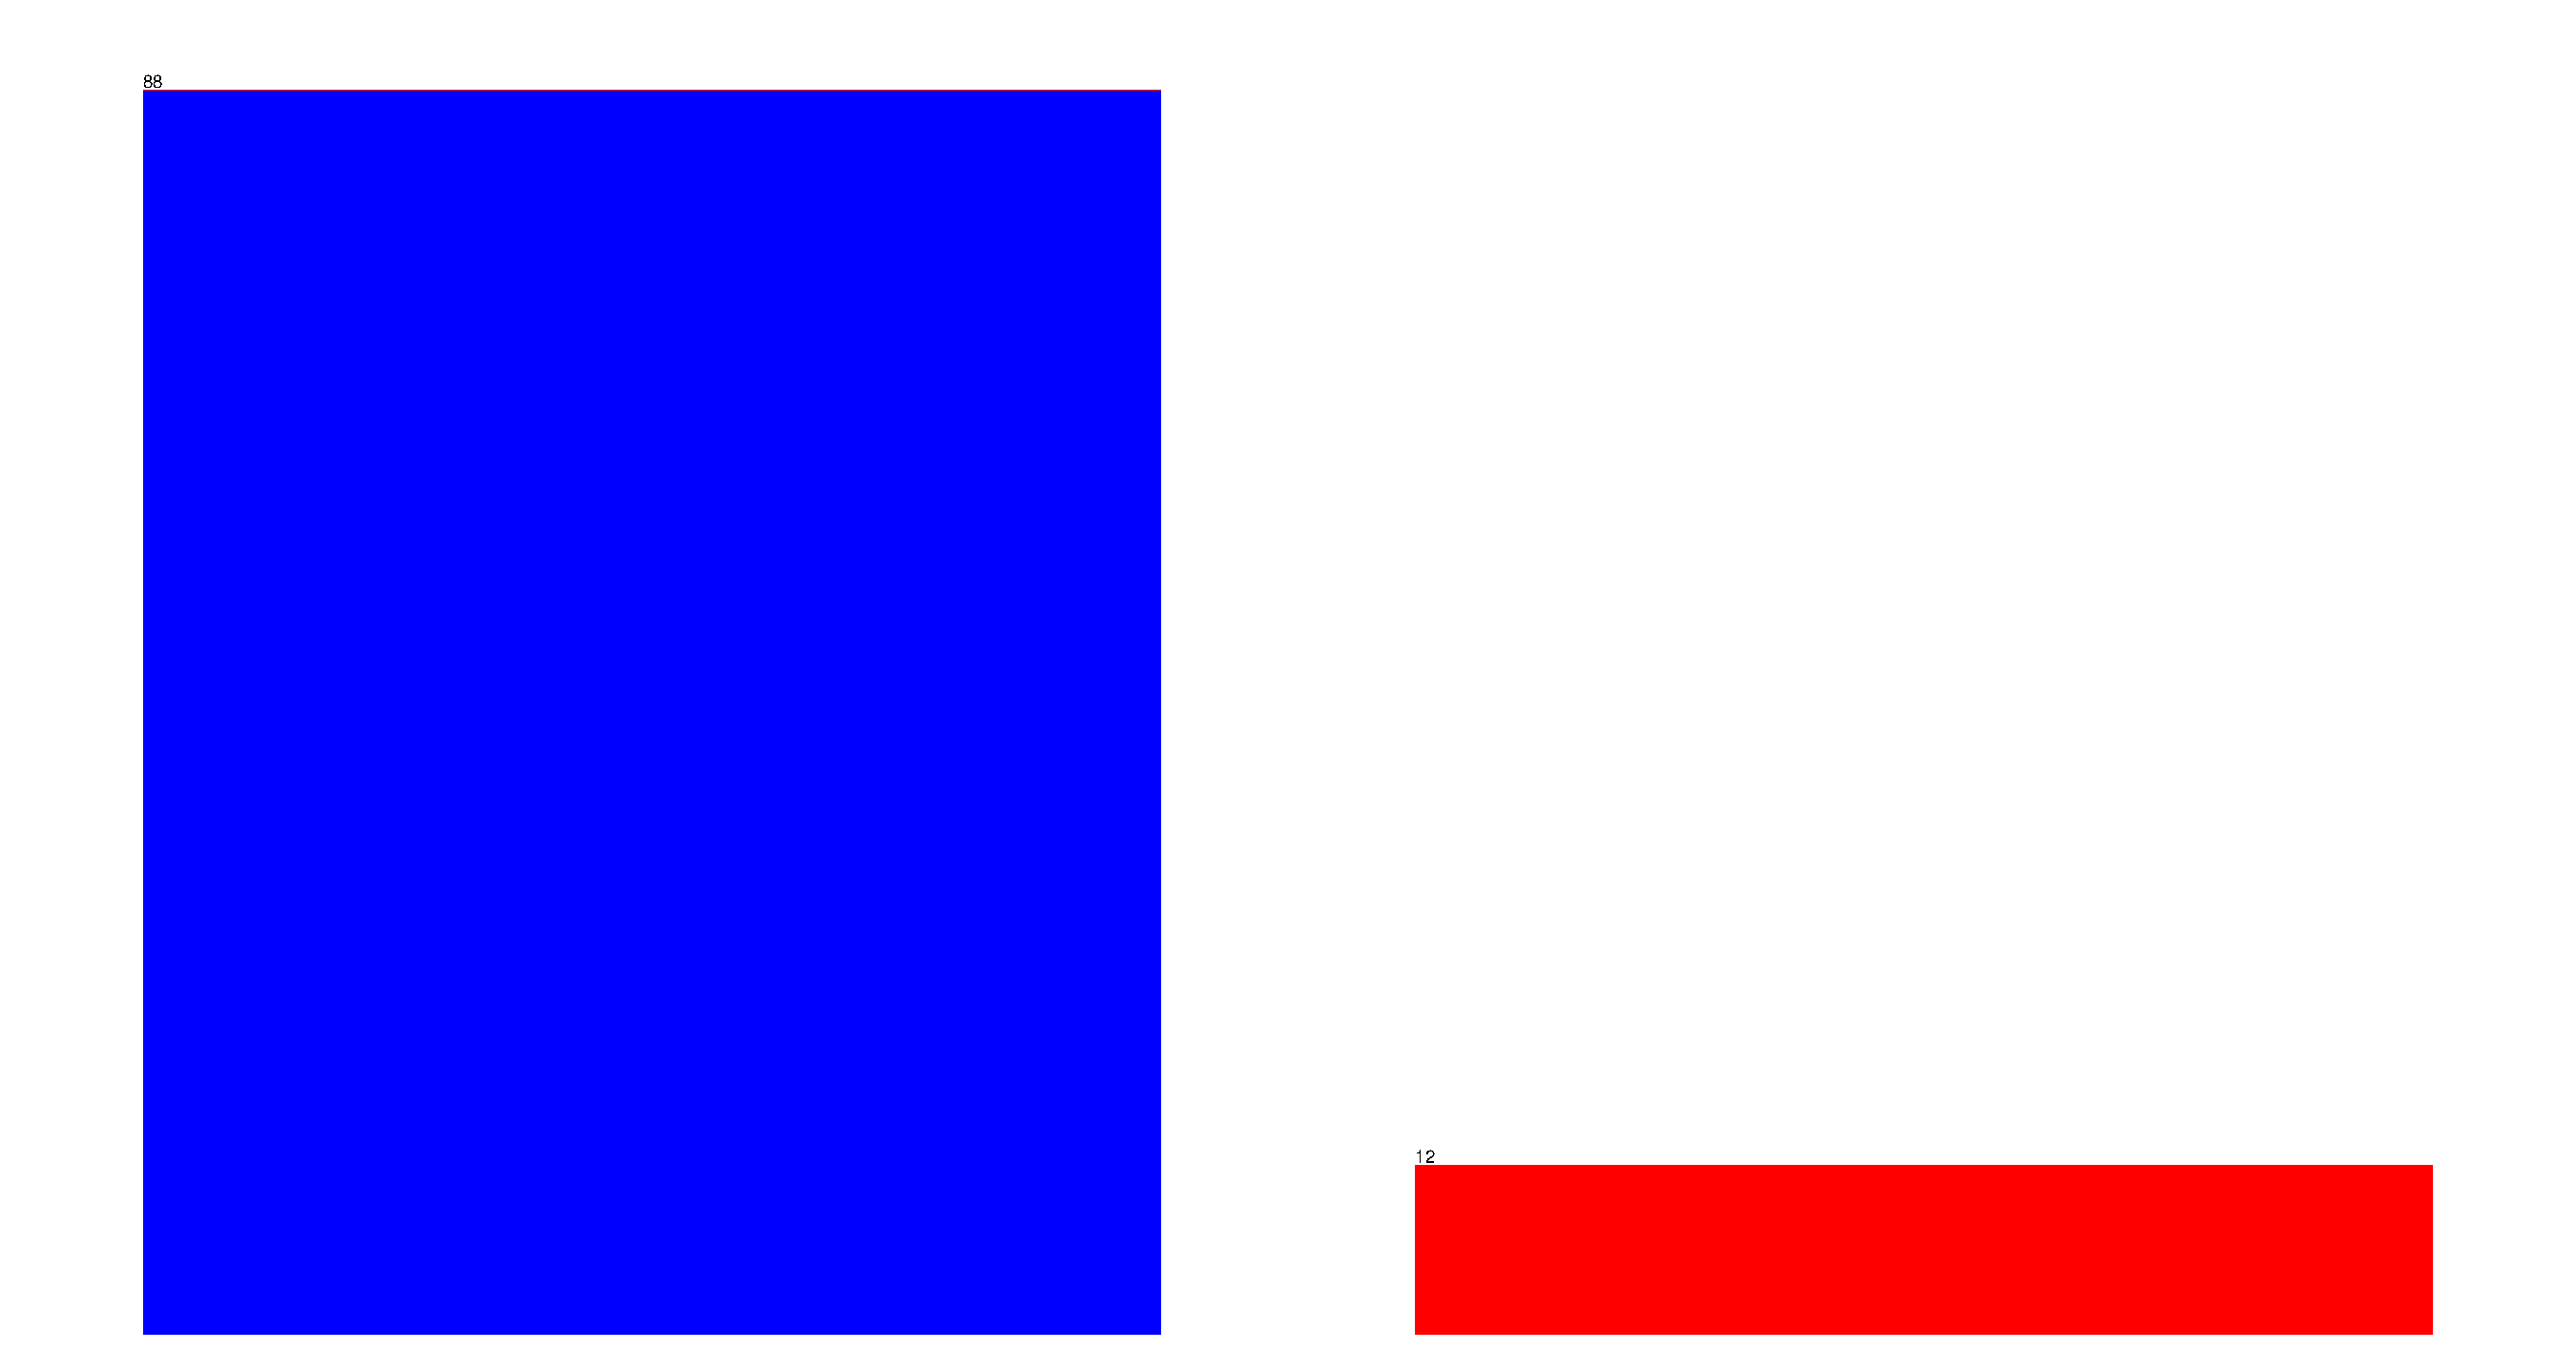
\includegraphics[width=0.85\textwidth]{fig/classes.eps}%
  \caption{%
    L'istogramma rappresenta i valori assunti dall'attributo classe:
    la colonna blu rappresenta le diagnosi di fertilità normale,
    quella rossa gli esami che evidenziano potenziali problematiche.
  }%
  \label{fig:classes}
\end{figure}

Questo disequilibrio tra le classi mette in difficoltà i modelli più semplici;
al fine di ottenere risultati validi, si è messo alla prova diverse configurazioni parametriche.

\todo[inline]{Aggiungere maggiori dettagli per ciascun attributo}

\subsection{Misure di performance dei classificatori}

\todo[inline]{Migliorare quanto segue}

Prima di partire con i vari dati, occorre però stabilire i criteri di misura delle performance dei vari classificatori:
a tale scopo ho tenuto conto in primo luogo della Confusion Matrix prodotta da ogni modello, successivamente dei valori di Precision e Recall per le classi in gioco, attribuendo un maggiore peso ai valori relativi alla classe ``O'' rispetto a ``N'' e infine del valore della ROC\@.
Come modalità di test ho scelto di applicare in ogni situazione la K-Fold Cross-Validation piuttosto che lo splitting statico dei dati in Training e Test Set, la motivazione dietro a questa scelta è l'esiguo numero di dati presenti nel dataset a cui si presta meglio una modalità come il K-Fold Cross-Validation,
in quanto pensata appositamente per dataset di piccole dimensioni.

\todo[inline]{Manca qualcosa?}

\subsection{kNN}
\subsection{Decision Tree}

La prima tecnica di classificazione testata è stata il Decision Tree.
In particolare, si è scelto di usare \texttt{J48}, implementazione dell'algoritmo \emph{C4.5};
esso realizza un albero binario a cui possono essere applicate tecniche di \emph{post pruning}
per ridurre le dimensioni dell'albero e l'errore commesso dal classificatore.

In primo luogo si è provato a generare un modello applicando i parametri standard impostati da Weka, ottenendo così i risultati riportati in~\Cref{fig:j48}.

\begin{figure}[H]
  \centering
  \adjincludegraphics[width=\linewidth,trim=0 0 0 {.3\height},clip]{fig/j48.eps}%
  \caption{Output di J48 eseguito tramite Weka}%
  \label{fig:j48}
\end{figure}

Com'è possibile notare, il classificatore costruisce un modello poco valido:
per quanto \emph{accuracy}, \emph{precision} e \emph{recall} per la classe ``\texttt{N}'' abbiano valori piuttosto elevati,
i corrispondenti per ``\texttt{O}'' risultano tendenti a \(0\).
Anche il valore di \emph{ROC}, indicatore principale della bontà di un modello di classificazione, risulta estremamente basso.

Osservando la struttura dell'albero costruito, è piuttosto chiaro il motivo di valori tanto bassi:
l'albero infatti è costruito da un'unica foglia i cui valori sono assegnati alla classe ``\texttt{N}'', causando così la situazione sopra descritta.

Ovviamente questo modello non risultava di una qualità soddisfacente, probabilmente a causa del post pruning,
il quale, in presenza di un tale sbilanciamento nella frequenza delle classi, tende a ridurre l'albero di classificazione a singola foglia.
Per porre rimedio a questa cosa si è provato ad aumentare e diminuire il parametro \texttt{confidenceFactor}, responsabile di accentuare o smussare le operazioni di pruning;
anche però variando questo parametro i risultati ottenuti non sono stati particolarmente differenti.

La situazione è decisamente migliorata disattivando il pruning (tramite parametro \texttt{unpruned}):
questa scelta ha finalmente prodotto un risultato notevolmente differente dai precedenti, come è possibile vedere in~\Cref{fig:j48-unpruned}.

\begin{figure}[H]
  \centering
  \begin{subfigure}{0.35\textwidth}
    \centering
    \adjincludegraphics[width=\linewidth,trim=0 {.37\height} {.55\width} {.25\height},clip]{fig/j48-unpruned.eps}%
    \label{fig:j48-unpruned:tree}
  \end{subfigure}
  \hfill
  \begin{subfigure}{0.6\textwidth}
    \centering
    \adjincludegraphics[width=\linewidth,trim=0 0 {.16\width} {.65\height},clip]{fig/j48-unpruned.eps}%
    \label{subfig:j48-unpruned:result}
  \end{subfigure}
  \caption{Albero di classificazione e output ottenuto con \texttt{J48} \emph{unpruned}}%
  \label{fig:j48-unpruned}
\end{figure}

Il risultato del classificatore è sicuramente migliore rispetto alla sua versione \emph{pruned}, tuttavia rimane ancora abbastanza insoddisfacente.

Sperimentando ulteriormente con la versione \emph{unpruned} di \texttt{J48},
abbassando il numero minimo di elementi per foglia a \texttt{1} il valore di \emph{recall} per la classe \texttt{O} e di \emph{True Positive} si alzava,
ma il valore di \emph{ROC} e \emph{precision} si abbassavano.

Si può dunque concludere che il classificatore \texttt{J48} non garantisce risultati ottimali sopra questo dataset, soprattutto a causa del grande sbilanciamento tra le distribuzioni delle classi.

Disabilitando il post pruning e abbassando il numero minimo di elementi per foglia a 1, si può classificare correttamente poco meno della metà degli elementi appartenente a \texttt{O}, classe più difficile da individuare ma allo stesso tempo più rilevante rispetto al dominio dei dati del sistema.

\subsection{Classificatori Bayesiani}
\subsection{Classificatori Lazy}
\subsection{Multi-Classificatori}
\subsubsection{Approccio Cost-Sensitive}
\subsubsection{Approccio Boosting}
\subsection{Rules}


\section{Conclusioni}

\end{document}
